
% xetex expected
\documentclass[xetex,professionalfont]{beamer}

% we want math
\usepackage{amsmath}

% fixes and extensions to amsmath
\usepackage{mathtools}

% additional math symbols
\usepackage{amssymb}

% good-looking fractions in text via \sfrac
\usepackage{xfrac}

% fix spaces after custom commands (see below for examples)
\usepackage{xspace}

% minted allows for fancy syntax highlighting (requires python with pygments)
% usage:
%   \begin{minted}{python}
%   codeb
%   \end{minted}
% \usepackage{minted}

% better looking tables
% usage:
%   begin with a \toprule, write a single row of column headings,
%   then add \midrule and after the columns of data we finish with \bottomrule
% example:
%   \begin{tabular}{llr} \toprule
%   Animal & Description & Price \midrule
%   cat & foo & 10 \\
%   dog & bar & 20 \\ \bottomrule
%   \end{tabular}
% note that good tables generally neither have vertical rules nor double rules
\usepackage{booktabs}

% system font support (requires xetex or luatex)
\usepackage{fontspec}
\setmonofont[Scale=0.7]{Cousine} % part of ttf-chromeos fonts on Arch

% multi-language quotes for babel
\usepackage{csquotes}

% easy way to include copyright information
\usepackage{copyrightbox}

% better bibliographies
\usepackage[backend=biber,style=authoryear]{biblatex}

% language support (english,ngerman)
\usepackage[english]{babel}

% -----------------------------------------------------------------------------

% specify PDF metadata
\hypersetup{pdftitle={CVSP VO - Introduction},pdfsubject={},pdfauthor={Christopher Pramerdorfer}}

% copyright font style
\makeatletter\renewcommand{\CRB@setcopyrightfont}{\tiny\color{lightgray}}

% add bib file
\addbibresource{literature.bib}

% use tuwcvl beamer theme
\usetheme{tuwcvl}

\usetikzlibrary{arrows}

% -----------------------------------------------------------------------------

% common english abbreviations
\newcommand{\ie}{\mbox{i.e.}\xspace} % i.e.
\newcommand{\eg}{\mbox{e.g.}\xspace} % e.g.

% math - argmin and argmax
\DeclareMathOperator*{\argmin}{arg\,min}
\DeclareMathOperator*{\argmax}{arg\,max}

% shortcuts for number ranges
\newcommand{\NN}{\mathbb{N}}
\newcommand{\ZZ}{\mathbb{Z}}
\newcommand{\QQ}{\mathbb{Q}}
\newcommand{\RR}{\mathbb{R}}

% bold vectors
\renewcommand{\vec}[1]{\ensuremath{\mathbf{#1}}}

% vector shortcuts
\newcommand{\va}{\vec{a}}
\newcommand{\vb}{\vec{b}}
\newcommand{\vc}{\vec{c}}
\newcommand{\ve}{\vec{e}}
\newcommand{\vr}{\vec{r}}
\newcommand{\vs}{\vec{s}}
\newcommand{\vt}{\vec{t}}
\newcommand{\vu}{\vec{u}}
\newcommand{\vv}{\vec{v}}
\newcommand{\vw}{\vec{w}}
\newcommand{\vx}{\vec{x}}
\newcommand{\vy}{\vec{y}}
\newcommand{\vz}{\vec{z}}

\newcommand{\pv}{\ensuremath{\boldsymbol{\theta}}}

% highlight
\newcommand{\highlight}[1]{\textcolor{tuwcvl_inf_red}{\textbf{#1}}}

% -----------------------------------------------------------------------------

\title{Computer Vision Systems Programming VO}
\subtitle{Introduction to Computer Vision}
\author{Christopher Pramerdorfer}
\institute{Computer Vision Lab, Vienna University of Technology}

\begin{document}

% -----------------------------------------------------------------------------

\begin{frame}
\maketitle
\end{frame}

% -----------------------------------------------------------------------------

\begin{frame}
\frametitle{Topics}

What is \emph{Computer Vision} (CV) and why is it important?\\\medskip
CV past, present, future\\\medskip
Relation to other research fields

\bigskip
\begin{center}
    \copyrightbox[b]
    {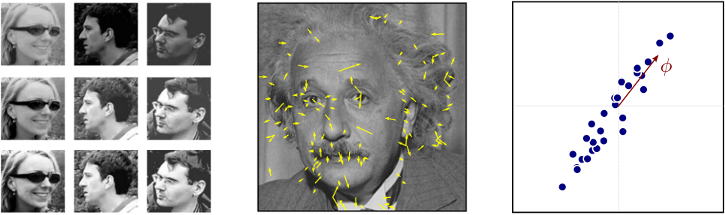
\includegraphics[width=8cm]{figures/intro-collage.png}}
    {\centering Images from \cite{lecun1989}, \cite{shotton2011}, \cite{taigman2013}}
\end{center}

\end{frame}

% -----------------------------------------------------------------------------

\begin{frame}
\frametitle{What Is CV and Why Is It Important?}

Let's hear what Fei-Fei Li has to say

\bigskip
\begin{center}
    \copyrightbox[b]
    {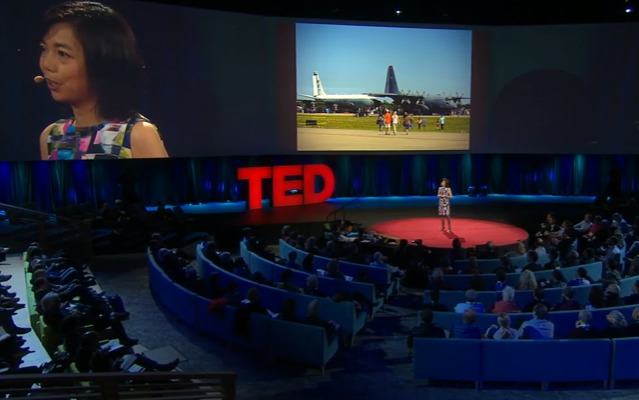
\includegraphics[width=7cm]{figures/feifei-ted.jpg}}
    {\centering Image from \href{https://www.ted.com/talks/fei_fei_li_how_we_re_teaching_computers_to_understand_pictures}{\texttt{ted.com}}}
\end{center}

\end{frame}

% -----------------------------------------------------------------------------

\begin{frame}
\frametitle{What Is CV and Why Is It Important?}

CV is about making computers understand images like humans do\\\medskip
Key to novel autonomous systems (cars, security, data analysis)\\\medskip
Tremendous progress in last decades, but still unsolved

\end{frame}

% -----------------------------------------------------------------------------

{
\setbeamertemplate{footline}{}
\begin{frame}

\begin{tikzpicture}[remember picture,overlay]
\fill[white] (current page.north west) rectangle (current page.south east);
\end{tikzpicture}

\end{frame}
}

% -----------------------------------------------------------------------------

\begin{frame}
\frametitle{CV Past, Present, Future}

CV research started around 50 years ago\\\medskip
Let's take a look at a few examples

\end{frame}

% -----------------------------------------------------------------------------

\begin{frame}
\frametitle{CV Past, Present, Future}
\framesubtitle{1963: Pose Estimation}

Edge-based pose estimation of polyhedra \\\medskip % based on relative orientation of edges
Among first CV applications % but not the first as often claimed, see Steve Seitz's slides

\bigskip
\begin{center}
    \copyrightbox[b]
    {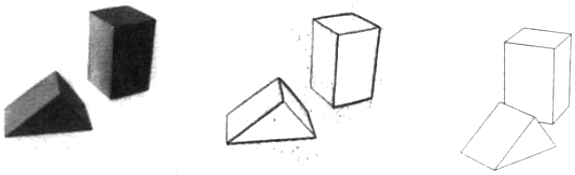
\includegraphics[width=7cm]{figures/blocks-world.png}} % input image, gradient-based edge detection, rendered objects from different viewpoint after recognition
    {\centering Image from \cite{roberts1963}}
\end{center}

\end{frame}

% -----------------------------------------------------------------------------

\begin{frame}
\frametitle{CV Past, Present, Future}
\framesubtitle{1973: Part-Based Object Detection}

Object representation as parts connected by springs\\\medskip % springs illustrate spatial relations
Known as pictorial structures or constellation models % can be solved in polynomial time via DP if the relation graph is a tree / still used today in improved form

\bigskip
\begin{center}
    \copyrightbox[b]
    {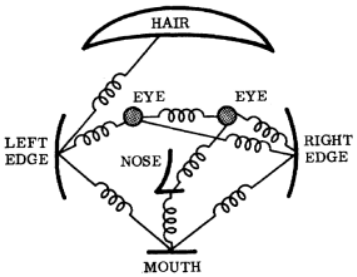
\includegraphics[width=4.5cm]{figures/constellation-model.png}}
    {\centering Image from \cite{fischler1973}}
\end{center}

\end{frame}

% -----------------------------------------------------------------------------

\begin{frame}
\frametitle{CV Past, Present, Future}
\framesubtitle{1989: OCR Using Convolutional Neural Networks}

% good article on DL history: http://www.wired.com/2014/01/geoffrey-hinton-deep-learning

Zip code recognition from images\\\medskip % from US postal service codes, manual preprocessing to obtain one image per digit
Among first applications using convolutional neural networks % but they had been proposed before, see LeCun's paper

\bigskip
\begin{center}
    \copyrightbox[b]
    {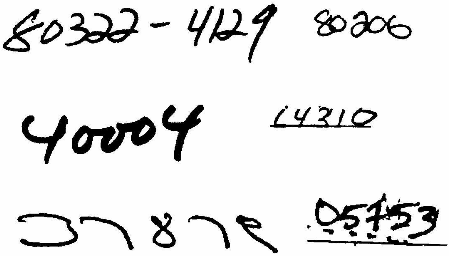
\includegraphics[width=4cm]{figures/zip-numbers.png}}
    {\centering Image from \cite{lecun1989}}
\end{center}

\end{frame}

% -----------------------------------------------------------------------------

\begin{frame}
\frametitle{CV Past, Present, Future}
\framesubtitle{1989: OCR Using Convolutional Neural Networks}

\begin{center}
    \copyrightbox[b]
    {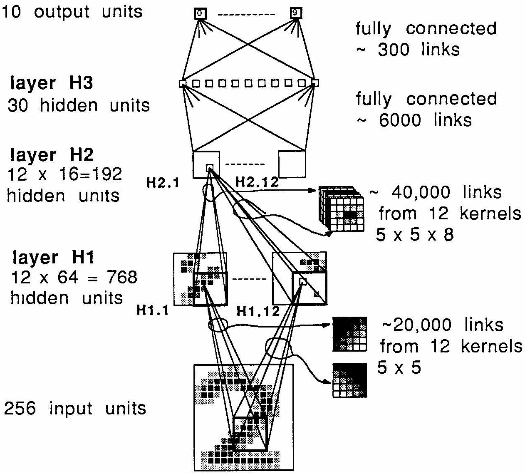
\includegraphics[width=6.5cm]{figures/zip-dnn.png}} % used network architecture. input is 16x16=256, h1 and h2 are convolutional, h3 and output are fully connected. 1256 units, ~65k connections, ~10k params in total
    {\centering Image from \cite{lecun1989}}
\end{center}

\end{frame}

% -----------------------------------------------------------------------------

\begin{frame}
\frametitle{CV Past, Present, Future}
\framesubtitle{1996: Image-Based Modeling}

Generate a 3D model from a set of images\\\medskip
Use this model and input images to render new images\\\medskip
\url{https://www.youtube.com/watch?v=RPhGEiM_6lM} % Facade introduced view-dependent texture mapping (select "best" images for texturing automatically based on similarity of current and image camera view), used for Matrix bullet-time shots according to video description

\bigskip
\begin{center}
    \copyrightbox[b]
    {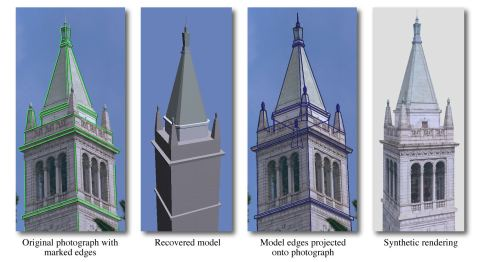
\includegraphics[width=6cm]{figures/facade.jpg}}
    {\centering Images from \cite{debevec1996}}
\end{center}

\end{frame}

% -----------------------------------------------------------------------------

\begin{frame}
\frametitle{CV Past, Present, Future}
\framesubtitle{2001: Real-Time Object Detection}

Fast object detection using Haar features and boosting\\\medskip % feature computation in constant time using integral images
Similar technologies used in smart cameras for auto focus

\bigskip
\begin{center}
    \copyrightbox[b]
    {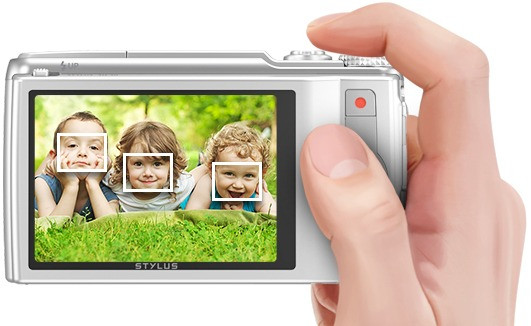
\includegraphics[width=6cm]{figures/camera-faces.jpg}}
    {\centering Image from \url{olympus-europa.com}}
\end{center}

\end{frame}

% -----------------------------------------------------------------------------

\begin{frame}
\frametitle{CV Past, Present, Future}
\framesubtitle{2006: Photo Tourism}

3D reconstruction from photo collections\\\medskip
Structure from Motion (SIFT + bundle adjustment) % these things were developed earlier

\bigskip
\begin{center}
    \copyrightbox[b]
    {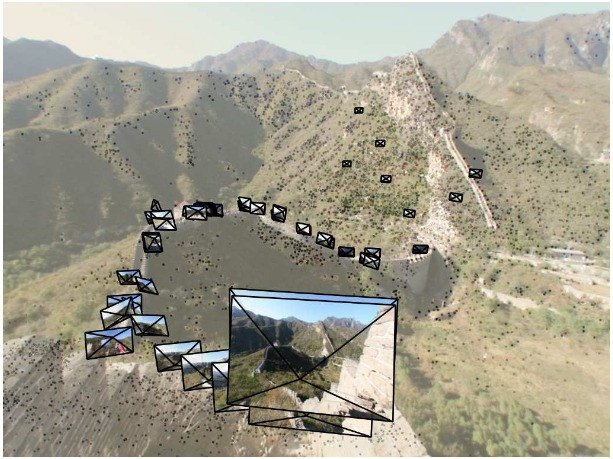
\includegraphics[width=5cm]{figures/photo-tourism.jpg}}
    {\centering Image from \cite{snavely2006}}
\end{center}

\end{frame}

% -----------------------------------------------------------------------------

\begin{frame}
\frametitle{CV Past, Present, Future}
\framesubtitle{2006: Photo Tourism -- Microsoft Photosynth}

\begin{center}
    \copyrightbox[b]
    {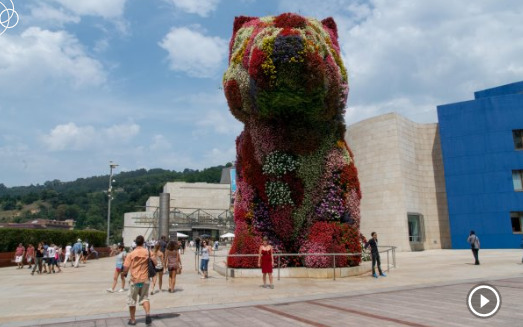
\includegraphics[width=7cm]{figures/photosynth.jpg}}
    {\centering Image from \href{https://photosynth.net/}{\texttt{photosynth.net}}}
\end{center}

\end{frame}

% -----------------------------------------------------------------------------

\begin{frame}
\frametitle{CV Past, Present, Future}
\framesubtitle{2006: Photo Tourism -- Building Rome in a Day}

\begin{center}
    \copyrightbox[b]
    {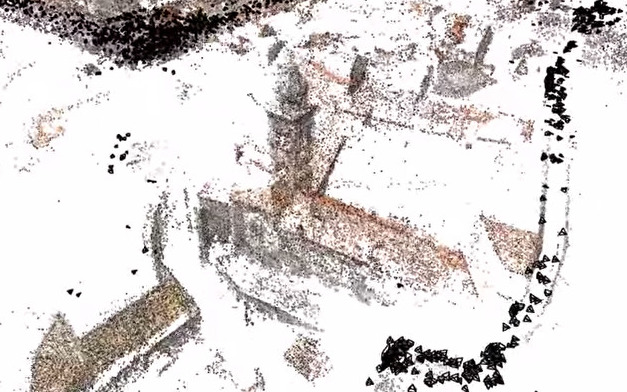
\includegraphics[width=7cm]{figures/dubrovnik.jpg}}
    {\centering Image from \url{https://www.youtube.com/watch?v=sQegEro5Bfo}}
\end{center}

\end{frame}

% -----------------------------------------------------------------------------

\begin{frame}
\frametitle{CV Past, Present, Future}
\framesubtitle{2011: Kinect}

Depth estimation via active stereo\\\medskip
Real-time pose estimation of multiple players

\bigskip
\begin{center}
    \copyrightbox[b]
    {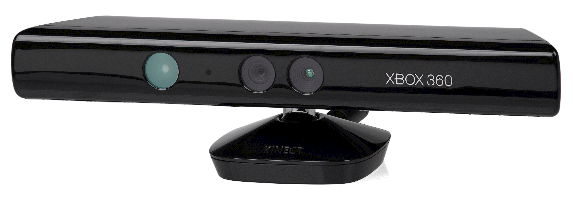
\includegraphics[width=5cm]{figures/kinect.png}}
    {\centering Image from \url{wikipedia.org}}
    \qquad
    \copyrightbox[b]
    {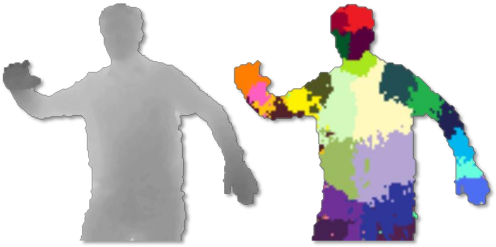
\includegraphics[width=4cm]{figures/kinect-pose.png}}
    {\centering Image from \cite{shotton2011}}
\end{center}

\end{frame}

% -----------------------------------------------------------------------------

\begin{frame}
\frametitle{CV Past, Present, Future}
\framesubtitle{2012: Deep Learning and Big Data}

Deep Learning on huge datasets for object recognition

\bigskip
\begin{center}
    \copyrightbox[b]
    {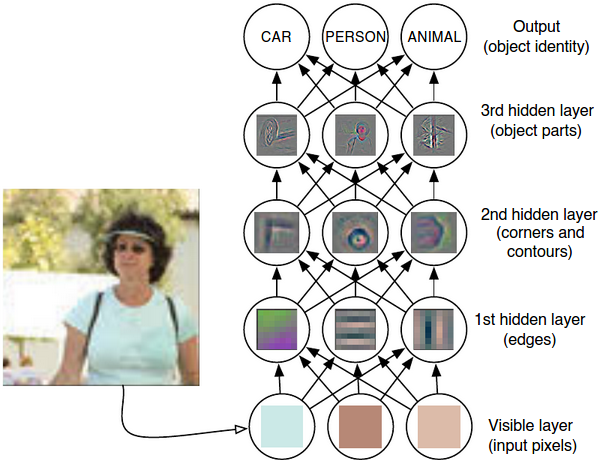
\includegraphics[width=6cm]{figures/dl-layer-example}}
    {\centering Image from \cite{bengio2015}}
\end{center}

\end{frame}

% -----------------------------------------------------------------------------

\begin{frame}
\frametitle{CV Past, Present, Future}
\framesubtitle{2012: Deep Learning and Big Data -- Clarifai}

% continue Fei-Fei Li's talk

\bigskip
\begin{center}
    \copyrightbox[b]
    {
\includegraphics[width=7cm]{figures/clarifai.jpg}}
    {\centering Image from \href{http://www.clarifai.com}{\texttt{clarifai.com}}}
\end{center}

\end{frame}

% -----------------------------------------------------------------------------

\begin{frame}
\frametitle{CV Past, Present, Future}
\framesubtitle{2012: Deep Learning and Big Data}

% continue Fei-Fei Li's talk

\bigskip
\begin{center}
    \copyrightbox[b]
    {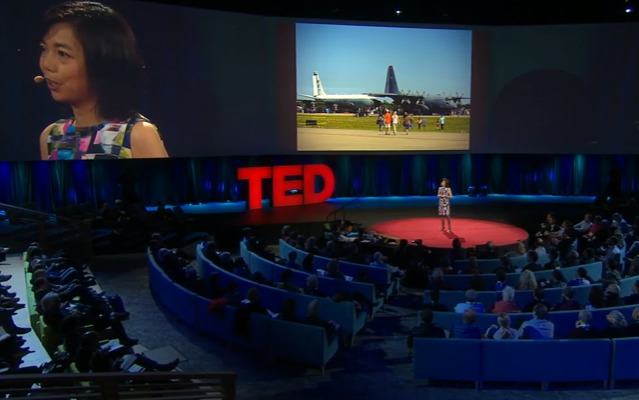
\includegraphics[width=7cm]{figures/feifei-ted.jpg}}
    {\centering Image from \href{https://www.ted.com/talks/fei_fei_li_how_we_re_teaching_computers_to_understand_pictures}{\texttt{ted.com}}}
\end{center}

\end{frame}

% -----------------------------------------------------------------------------

\begin{frame}
\frametitle{CV Past, Present, Future}
\framesubtitle{20xx: Human-Level Object Recognition}

Object recognition without constraints % like occlusions, perspective, background

\bigskip
\begin{center}
    \copyrightbox[b]
    {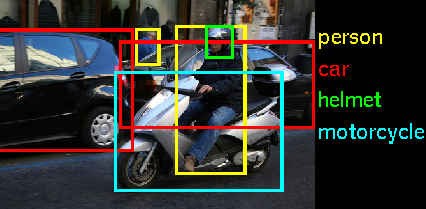
\includegraphics[width=6cm]{figures/object-detection.png}}
    {\centering Image from \url{image-net.org}}
\end{center}

\end{frame}

% -----------------------------------------------------------------------------

\begin{frame}
\frametitle{CV Past, Present, Future}
\framesubtitle{20xx: Autonomous Cars}

Cars that drive autonomously\\\medskip
\url{https://www.youtube.com/watch?v=bDOnn0-4Nq8}

\bigskip
\begin{center}
    \copyrightbox[b]
    {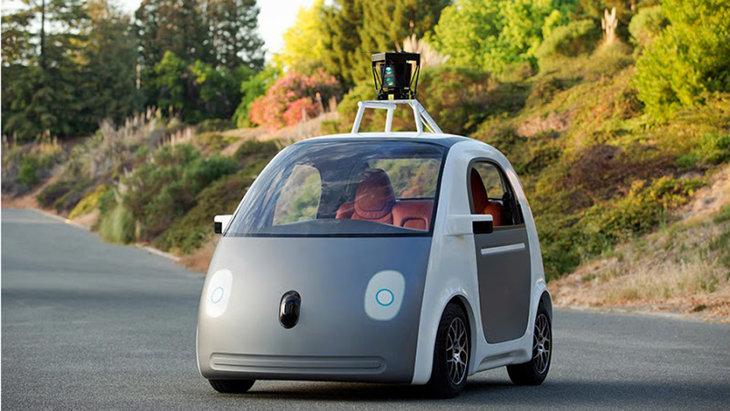
\includegraphics[width=6cm]{figures/google-car.jpg}}
    {\centering Image by Google}
\end{center}

\end{frame}

% -----------------------------------------------------------------------------

\begin{frame}
\frametitle{CV Past, Present, Future}
\framesubtitle{20xx: Human-Level Vision}

Segmentation, context, motion, emotions

\bigskip
\begin{center}
    \copyrightbox[b]
    {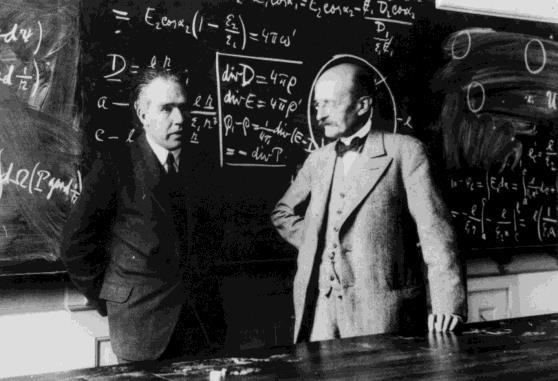
\includegraphics[width=6cm]{figures/planck-bohr.png}}
    {\centering Image from Larry Zitnick's slides}
\end{center}

\end{frame}

% -----------------------------------------------------------------------------

\begin{frame}
\frametitle{CV Past, Present, Future}
\framesubtitle{20xx: Human-Level Vision}

% continue Fei-Fei Li's talk

\bigskip
\begin{center}
    \copyrightbox[b]
    {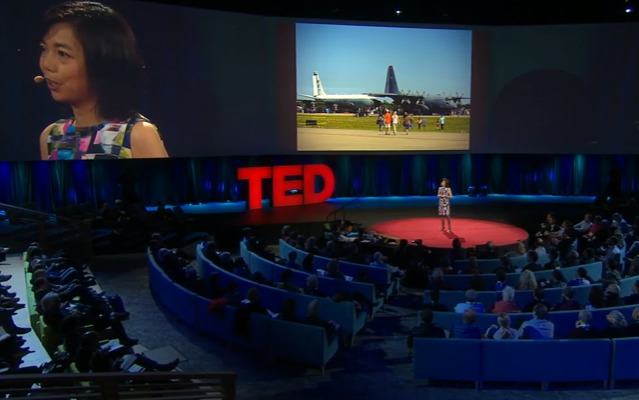
\includegraphics[width=7cm]{figures/feifei-ted.jpg}}
    {\centering Image from \href{https://www.ted.com/talks/fei_fei_li_how_we_re_teaching_computers_to_understand_pictures}{\texttt{ted.com}}}
\end{center}

\end{frame}

% -----------------------------------------------------------------------------

{
\setbeamertemplate{footline}{}
\begin{frame}

\begin{tikzpicture}[remember picture,overlay]
\fill[white] (current page.north west) rectangle (current page.south east);
\end{tikzpicture}

\end{frame}
}

% -----------------------------------------------------------------------------

\begin{frame}
\frametitle{CV and Related Fields}

In other lectures you probably heard about
\begin{itemize}
    \item Mathematics and statistics
    \item Image processing (e.g.\ linear filtering, SIFT)
    \item Machine learning (e.g.\ SVM)
\end{itemize}

\bigskip
Let's see how CV and these fields are related
\begin{itemize}
    \item Using an example application for explanation purposes
\end{itemize}

\end{frame}

% -----------------------------------------------------------------------------

\begin{frame}
\frametitle{CV and Related Fields}
\framesubtitle{Example Application}

We want to distinguish two kinds of fish in images
\begin{itemize}
    \item Each image contains exactly one fish
    \item Only fishes of two known kinds (e.g.\ sea bass and salmon) % from Duda's book
    \item Little background clutter
\end{itemize}

\bigskip
This is a binary (two-class) \emph{image classification} problem

\end{frame}

% -----------------------------------------------------------------------------

\begin{frame}
\frametitle{CV and Related Fields}
\framesubtitle{Formal Definition of CV}

CV is about making computers understand images like humans do

\bigskip
So in mathematical terms CV is about
\begin{itemize}
    \item Inferring some world state (a scalar $w$ or vector $\vw$)
    \item From measurements $\vx$ (a \emph{feature vector})
\end{itemize}

\end{frame}

% -----------------------------------------------------------------------------

\begin{frame}
\frametitle{CV and Related Fields}
\framesubtitle{Example Application}

$w$ encodes what we care about, the fish type
\begin{itemize}
    \item Let $w=0$ if the image depicts a sea bass
    \item Let $w=1$ if the image depicts a salmon
\end{itemize}

\bigskip
What are our measurements $\vx$?
\begin{itemize}
    \item We could simply use the whole image
    \item But we should be able to come up with something better
    \item This is where image processing comes in
\end{itemize}

\end{frame}

% -----------------------------------------------------------------------------

\begin{frame}
\frametitle{CV and Related Fields}
\framesubtitle{Image Processing}

We use \emph{image processing} to extract $\vx$ from images
\begin{itemize}
    \item Preprocessing step for CV
\end{itemize}

\bigskip
Different problems favor different features $\vx$

\bigskip
Do sea basses and salmons look differently?
\begin{itemize}
    \item $\vx$ should encode fish appearance
\end{itemize}

\bigskip
Do they differ in size?
\begin{itemize}
    \item $\vx$ should encode fish size
\end{itemize}

\end{frame}

% -----------------------------------------------------------------------------

\begin{frame}
\frametitle{CV and Related Fields}
\framesubtitle{Statistics}

How do we get from $\vx$ to $\vw$?
\begin{itemize}
    \item This is what CV is all about!
\end{itemize}

\bigskip
CV is about describing the relationship between $\vx$ and $\vw$
\begin{itemize}
    \item This relationship is called \emph{model}
\end{itemize}

\bigskip
Put simply, there are two ways for \emph{modeling} this relationship
\begin{itemize}
    \item Statistically by looking at data and using domain knowledge
    \item Using a generic machine learning algorithm
\end{itemize}

\bigskip
More on models later

\end{frame}

% -----------------------------------------------------------------------------

\begin{frame}
\frametitle{CV and Related Fields}
\framesubtitle{Mathematics}

Models are mathematical functions $\Gamma:\vx\mapsto\vw$ % i just use gamma here but this is just a personal choice

\bigskip
Models have parameters that are \emph{learned} from data
\begin{itemize}
    \item This is a \emph{mathematical optimization} problem
\end{itemize}

\end{frame}

% -----------------------------------------------------------------------------

\begin{frame}
\frametitle{CV and Related Fields}
\framesubtitle{Machine Learning}

\emph{Machine Learning} (ML) studies techniques for learning from data
\begin{itemize}
    \item Namely algorithms for learning and inference
    \item So any CV model that involves learning is a ML technique
\end{itemize}

\bigskip
Generic ML algorithms (e.g.\ SVM) are often used as the model % unless we know the physical relationship between x and v e.g. structure from motion, tracking with sensor noise

\bigskip
Strictly speaking, models and algorithms are not the same
\begin{itemize}
    \item More on this later
\end{itemize}

\end{frame}

% -----------------------------------------------------------------------------

\begin{frame}[allowframebreaks=0.9]
\frametitle{Bibliography}

\printbibliography

\end{frame}

\end{document}
